% ----------------------------------------------------------------------------
\section{Features}
\label{protofeatures}
This section describes which features are supported by the chat protocol.
Figure \ref{features-technologies} gives a quick overview of how the
features relate to the used technologies.
\begin{figure}
    \centering
    \caption{Features and Technologies}
    \label{features-technologies}
    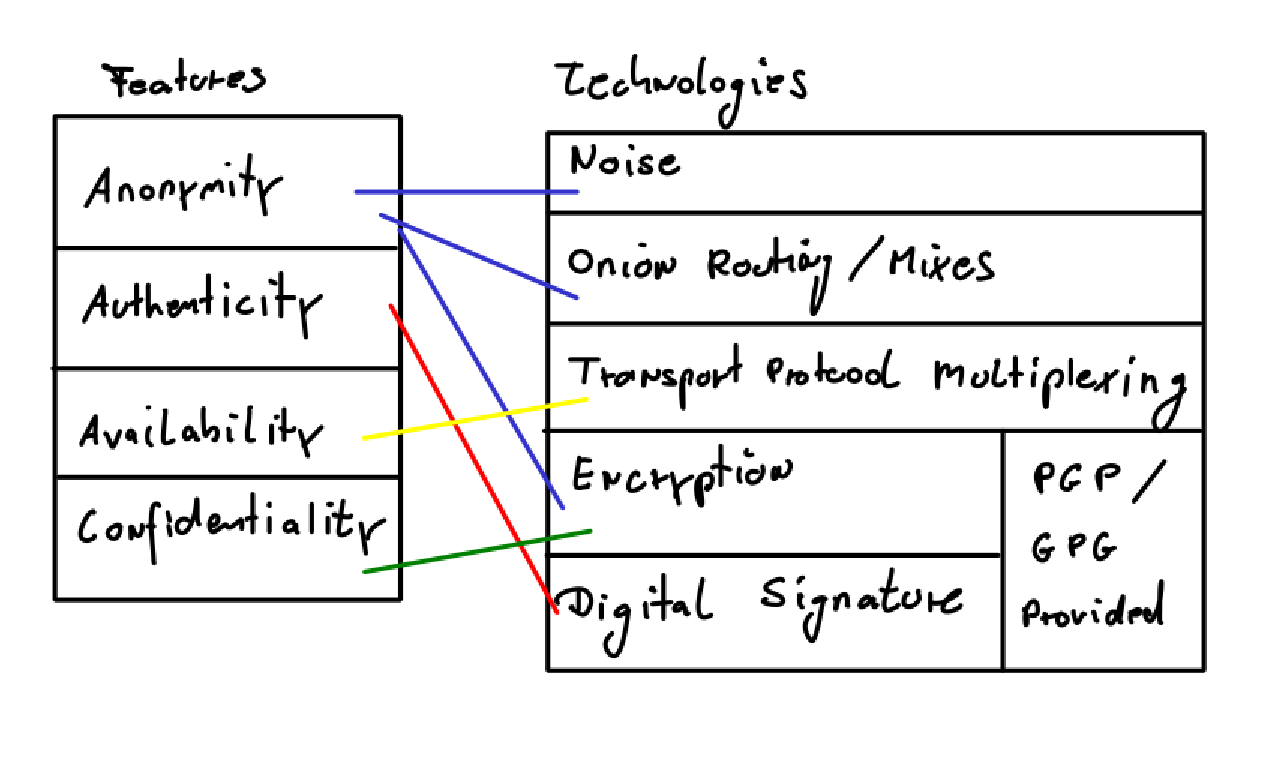
\includegraphics[scale=0.8]{features-technologies.eps}
\end{figure}
% ----------------------------------------------------------------------------
\subsection{Anonymity}
One of the main objectives of this protocol is to provide a chat system that
hides who is talking to whom (\textit{Sender-Receiver Anonymity}). 
In practise there are limits on the degree of anonymity that can be reached.
This protocol specifies the use of
\begin{itemize}
\item Onion Routing (\ref{onionrouting}, p. \pageref{onionrouting}),
\item Noise (\ref{noise}, p. \pageref{noise})
\item and OpenPGP (\ref{openpgp}, p. \pageref{openpgp})
\end{itemize}
to achieve a high degree of anonymity.
% ----------------------------------------------------------------------------
\subsubsection{Degree of Anonymity}
\label{degreeofanonymity}
If an attacker controls all hosts that are part of the chat network, 
it is impossible to guarantee anonymity at all.
Thus to allow any degree of anonymity, there must be hosts in the network,
which are not run by the attacker besides the sender and the receiver.
As specified by Onion Routing, there are a number of proxy peers used
to hide the message receiver.

In a network in which the attacker does not run all nodes, there is a probability
that the given route considers only the hosts run by the attacker. As soon as the
route considers at least one different host, the attacker cannot distinguish
between the real recipient and a proxy peer. So we have to consider the probability
that the attacker controls \textbf{all} proxy peers for a given route only.
This probability is the same as the one used to calculate the winning probability
in the game of luck \textit{Lotto}, in which the
winning chances are expressed like this:
$$P_r = \frac{{\binom{6}{r}}{\binom{N-6}{6-r}}}{{\binom{N}{6}}}, r \in \{0, \ldots, 6\}$$
%To remove anonymity, all peers in a route, which are not the 
%sender and the receiver have to be compromised.
Depending on the number of hosts in a network (number of possible
numbers in lotto) and on the number of hosts in a specific route
(number of correct numbers in lotto), the de-anonymisation
probabilities (lotto: winning probabilities) are shown in table \ref{deanontable}.
\begin{longtable}{|c|c|c|c|c|c|}
\caption{De-Anonymisation Probablities (for one packet)}
\label{deanontable}\\
\hline
\textbf{Peers in network /} & \textbf{$10$} & \textbf{$10^2$} & \textbf{$10^3$} & \textbf{$10^4$} & \textbf{$10^5$} \\
\textbf{Proxy peers} & & & & & \\
\hline
\textbf{1} & 1:10 & 1:100 & 1:1000 & 1:10000 & 1:100000\\
\hline
\textbf{2} & 1:45 & 1:4950 & 1:499500 & 1:4.9995e+07 & 1:4.99995e+09\\
\hline
\textbf{3} & 1:120 & 1:161700 & 1:1.66167e+08 & 1:1.66617e+11 & 1:1.66662e+14\\
\hline
\textbf{4} & 1:210 & 1:3.92122e+06 & 1:4.14171e+10 & 1:4.16417e+14 & 1:4.16642e+18\\
\hline
\textbf{5} & 1:252 & 1:7.52875e+07 & 1:8.25029e+12 & 1:8.325e+17 & 1:8.3325e+22\\
\hline
\textbf{6} & 1:210 & 1:1.19205e+09 & 1:1.36817e+15 & 1:1.38681e+21 & 1:1.38868e+27\\
\hline
\textbf{7} & 1:120 & 1:1.60076e+10 & 1:1.94281e+17 & 1:1.97996e+24 & 1:1.98371e+31\\
\hline
\textbf{8} & 1:45 & 1:1.86088e+11 & 1:2.41151e+19 & 1:2.47322e+27 & 1:2.47946e+35\\
\hline
\textbf{9} & 1:10 & 1:1.90223e+12 & 1:2.65802e+21 & 1:2.74583e+30 & 1:2.75474e+39\\
\hline
\textbf{10} & 1:1 & 1:1.73103e+13 & 1:2.6341e+23 & 1:2.74336e+33 & 1:2.75449e+43\\
\hline
\end{longtable}
As can be seen in this table, the probability of an attacker being able to
de-anonymise in a network of 100 peers using 5 proxy peers is less then
the probability of winning Lotto with 6 of 49 (1:13983816).
To support a high chance of not hitting the attackers peers and thus
avoiding de-anonymisation, the number of peers in the network as well 
as the number of proxy peers should be increased as much as possible. 
The number of peers in the network are
depending on how many peers are actually using the network. This can be
increased to a certain degree by adding artificial peers.
The number of proxy peers cannot be increased infinitely, 
as shown in \ref{latency}, p. \pageref{latency}.
% ----------------------------------------------------------------------------
\subsection{Authenticity and Confidentiality}
Digital signatures provide methods to ensure that a given message
was composed by a given public key and that the content has not been
modified. 
The process of encryption protects data from external
viewing and thus ensures the confidentiality of a message.
The features of OpenPGP (\ref{openpgp}, p. \pageref{openpgp})
are being used to guarantee authenticity.
% ----------------------------------------------------------------------------
\subsection{Availability}
To prevent easy denial of service attacks, this protocol specifies various
measurements to make denial of service attacks harder. In particular
the following techniques are used to support the availbility:
\begin{itemize}
\item Transport protocol multiplexing (\ref{multiplexing}, p. \pageref{multiplexing})
\item Transport protocol tunneling (\ref{tunneling}, p. \pageref{tunneling})
\end{itemize}

\subsubsection{Steganographic}
Not for hiding, but to support longer überleben?
http is pretty well suited for this.
mixing with smtp, imap, pop3, tcp. etc.

FIXME 

% ----------------------------------------------------------------------------
\subsection{Direct chat}
This chat protocol supports only direct chat (1:1) as opposed 
to multi user / group chat.
% ----------------------------------------------------------------------------
\section{Summary}
\begin{enumerate}
% FIXME: enable this one?
%\item Nobody, but the intended receiver(s) know(s) \emph{that} you wrote a message.
\item Nobody, but the intended receiver(s) can view the \emph{message content}.
\item Nobody, but the intended receiver(s) can \emph{verify} the source of the message being you.
\item Nobody, but the intended receiver(s) know(s) \emph{who} the message was sent to.
\item The network must survive attacks of a single attacker.
%\item Hard (if not practilcally impossible) to block chatting.
\end{enumerate}
FIXME 
